\documentclass[tikz,border=12pt]{standalone}
\usepackage[T1]{fontenc}
\usepackage{mathpazo}
\usepackage{amsmath,amssymb}
\usetikzlibrary{arrows.meta, positioning, calc, fit}

\definecolor{stblue}{HTML}{7B97AD}
\definecolor{rwgold}{HTML}{B8995E}
\definecolor{sage}{HTML}{7A9A7E}
\definecolor{dkbrown}{HTML}{3D3530}
\definecolor{wmgray}{HTML}{7B7067}
\definecolor{cream}{HTML}{F9F6F0}
\definecolor{border}{HTML}{D4C9B8}

\begin{document}
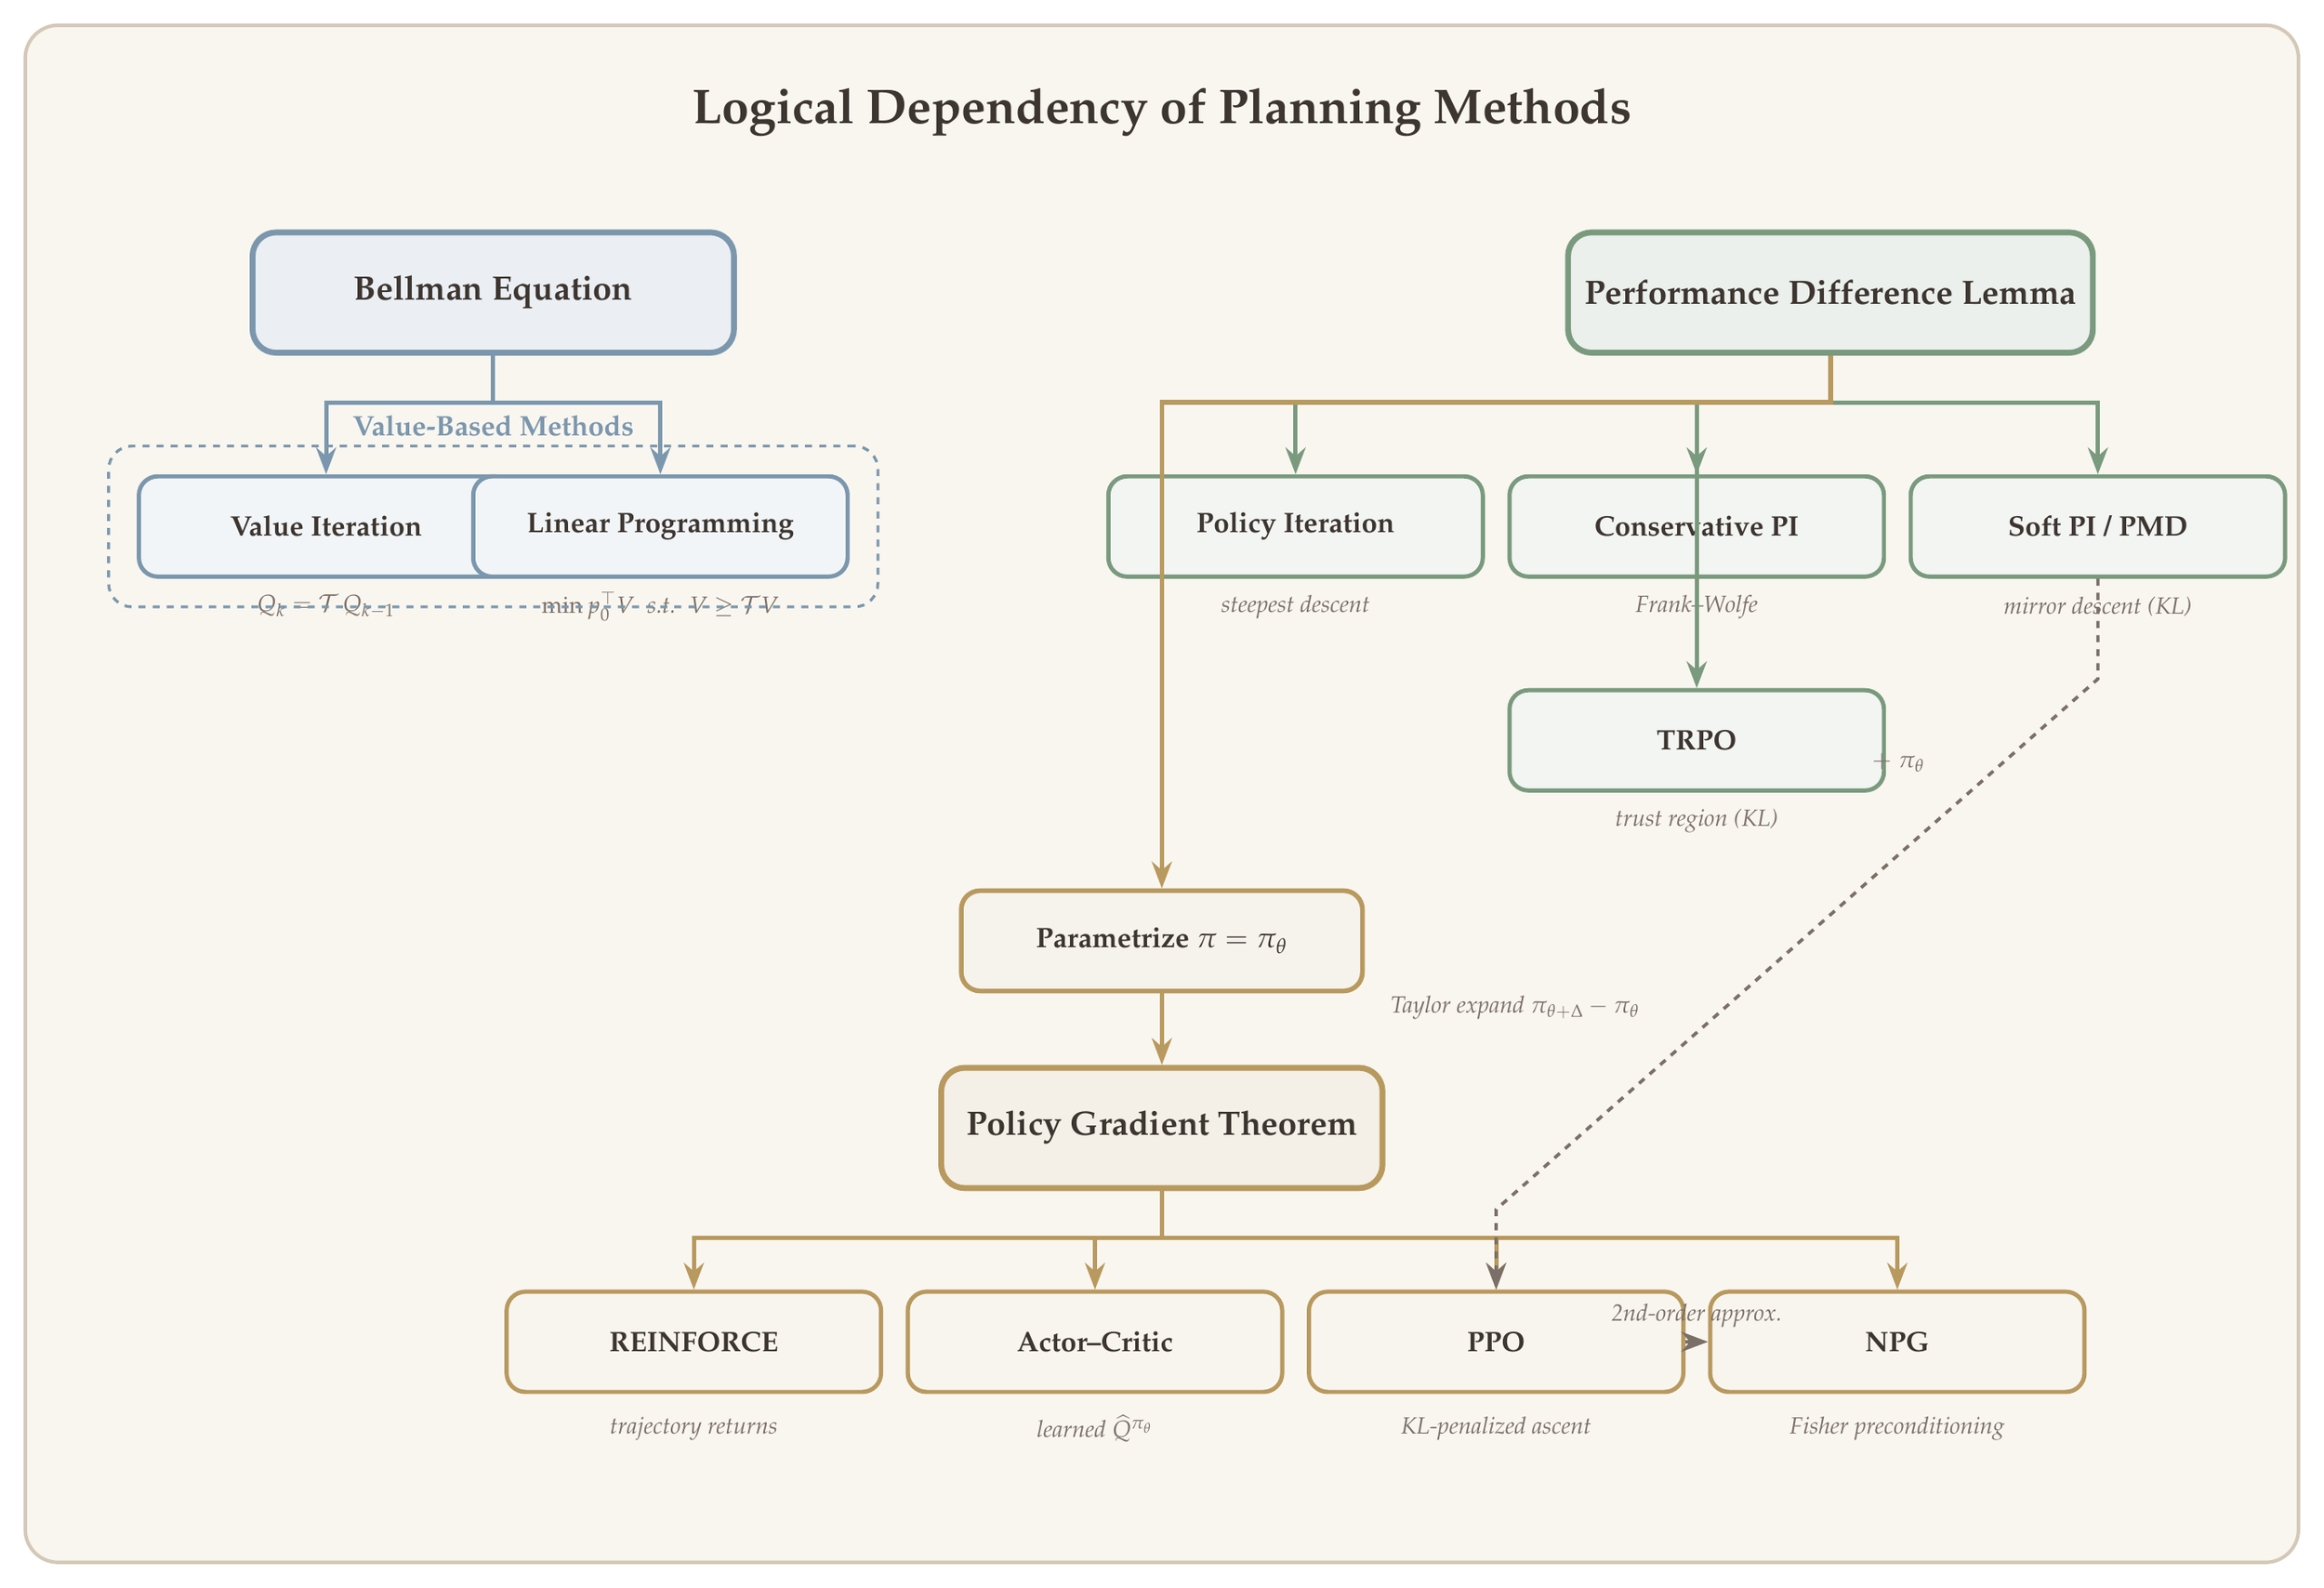
\begin{tikzpicture}[
  >={Stealth[length=4mm, width=3mm]},
  foundation/.style={draw=#1, line width=2.5pt, fill=#1!15, rounded corners=10pt,
    minimum width=72mm, minimum height=18mm, font=\Large\bfseries, text=dkbrown,
    align=center, inner sep=7pt},
  method/.style={draw=#1, line width=1.8pt, fill=#1!10, rounded corners=8pt,
    minimum width=56mm, minimum height=15mm, font=\large\bfseries, text=dkbrown,
    align=center, inner sep=6pt},
  optlabel/.style={font=\normalsize\itshape, text=wmgray, align=center},
  arr/.style={->, line width=1.8pt, #1},
  darr/.style={->, line width=1.4pt, dashed, #1},
]

% Background
\fill[cream, rounded corners=14pt] (-8.5,-15.5) rectangle (25.5,7.5);
\draw[border, rounded corners=14pt, line width=1.5pt] (-8.5,-15.5) rectangle (25.5,7.5);

% Title
\node[font=\huge\bfseries, text=dkbrown] at (8.5,6.2)
  {Logical Dependency of Planning Methods};

% =============================================
% Top level: Two theoretical foundations
% =============================================
\node[foundation=stblue] (bellman) at (-1.5,3.5)
  {Bellman Equation};

\node[foundation=sage] (pdl) at (18.5,3.5)
  {Performance Difference Lemma};

% =============================================
% Value-based methods (left branch)
% =============================================
\node[method=stblue] (vi) at (-4.0,0.0) {\textbf{Value Iteration}};
\node[method=stblue] (lp) at (1.0,0.0) {\textbf{Linear Programming}};

\draw[arr=stblue] (bellman.south) -- ++(0,-0.7) -| (vi.north);
\draw[arr=stblue] (bellman.south) -- ++(0,-0.7) -| (lp.north);

\node[optlabel] at (-4.0,-1.2) {$Q_k = \mathcal{T}\, Q_{k-1}$};
\node[optlabel] at (1.0,-1.2) {$\min p_0^\top V$\; s.t.\; $V \geq \mathcal{T}V$};

% Value-based dashed box
\node[draw=stblue, line width=1.2pt, dashed, rounded corners=10pt,
  fit=(vi)(lp), inner sep=12pt,
  label={[font=\large\bfseries, text=stblue]above:Value-Based Methods}] {};

% =============================================
% Policy-based methods from PDL
% =============================================
\node[method=sage] (pi) at (10.5,0.0) {\textbf{Policy Iteration}};
\node[method=sage] (cpi) at (16.5,0.0) {\textbf{Conservative PI}};
\node[method=sage] (spi) at (22.5,0.0) {\textbf{Soft PI / PMD}};

\draw[arr=sage] (pdl.south) -- ++(0,-0.7) -| (pi.north);
\draw[arr=sage] (pdl.south) -- ++(0,-0.7) -| (cpi.north);
\draw[arr=sage] (pdl.south) -- ++(0,-0.7) -| (spi.north);

\node[optlabel] at (10.5,-1.2) {steepest descent};
\node[optlabel] at (16.5,-1.2) {Frank--Wolfe};
\node[optlabel] at (22.5,-1.2) {mirror descent (KL)};

% TRPO
\node[method=sage] (trpo) at (16.5,-3.2) {\textbf{TRPO}};
\draw[arr=sage] (pdl.south) -- ++(0,-0.7) -| (16.5,-0.85) -- (trpo.north);
\node[optlabel] at (16.5,-4.4) {trust region (KL)};

% =============================================
% Parametrization bridge
% =============================================
\node[draw=rwgold, line width=2pt, fill=rwgold!12, rounded corners=8pt,
  minimum width=60mm, minimum height=15mm, font=\large\bfseries, text=dkbrown]
  (param) at (8.5,-6.2) {Parametrize $\pi = \pi_\theta$};

\draw[arr=rwgold, line width=2pt] (pdl.south) -- ++(0,-0.7) -| (8.5,-1.0) -- (param.north);

\node[optlabel, anchor=west] at (11.8,-7.2)
  {Taylor expand $\pi_{\theta+\Delta} - \pi_\theta$};

% PG theorem
\node[foundation=rwgold, minimum width=66mm] (pgt) at (8.5,-9.0)
  {Policy Gradient Theorem};

\draw[arr=rwgold, line width=2pt] (param.south) -- (pgt.north);

% =============================================
% PG-based methods (bottom row)
% =============================================
\node[method=rwgold] (reinforce) at (1.5,-12.2) {\textbf{REINFORCE}};
\node[method=rwgold] (ac) at (7.5,-12.2) {\textbf{Actor--Critic}};
\node[method=rwgold] (ppo) at (13.5,-12.2) {\textbf{PPO}};
\node[method=rwgold] (npg) at (19.5,-12.2) {\textbf{NPG}};

\draw[arr=rwgold] (pgt.south) -- ++(0,-0.7) -| (reinforce.north);
\draw[arr=rwgold] (pgt.south) -- ++(0,-0.7) -| (ac.north);
\draw[arr=rwgold] (pgt.south) -- ++(0,-0.7) -| (ppo.north);
\draw[arr=rwgold] (pgt.south) -- ++(0,-0.7) -| (npg.north);

\node[optlabel] at (1.5,-13.5) {trajectory returns};
\node[optlabel] at (7.5,-13.5) {learned $\widehat{Q}^{\pi_\theta}$};
\node[optlabel] at (13.5,-13.5) {KL-penalized ascent};
\node[optlabel] at (19.5,-13.5) {Fisher preconditioning};

% =============================================
% Dashed connections
% =============================================
% SPI -> PPO
\draw[darr=wmgray] (spi.south) -- ++(0,-1.5) -- ($(ppo.north)+(0,1.2)$) -- (ppo.north);
\node[optlabel, anchor=south west] at (19.0,-3.8) {$+\;\pi_\theta$};

% NPG approximates PPO
\draw[darr=wmgray] (ppo.east) -- (npg.west)
  node[midway, above=2pt, font=\normalsize\itshape, text=wmgray] {2nd-order approx.};

\end{tikzpicture}
\end{document}
